
\section{\label{part:5}Synthèse}
\begin{obj}
Analyser et comparer les deux solutions technologiques étudiées précédemment pour concevoir le stabilisateur
\end{obj}

\ifprof
\else

Une simulation numérique a été effectuée afin d'analyser la capacité des deux solutions technologiques à vérifier l'exigence 1.2.1 relative au filtrage du mouvement. Pour cela, la réponse harmonique de la fonction $Z_{G}(p) / Z_{\text {pert }}(p)$ obtenue pour le système avec commande active est comparée à celle obtenue avec le système par filtrage passif dont le modèle a été linéarisé (figure~\ref{fig:15}).

\begin{figure}[H]
\centering
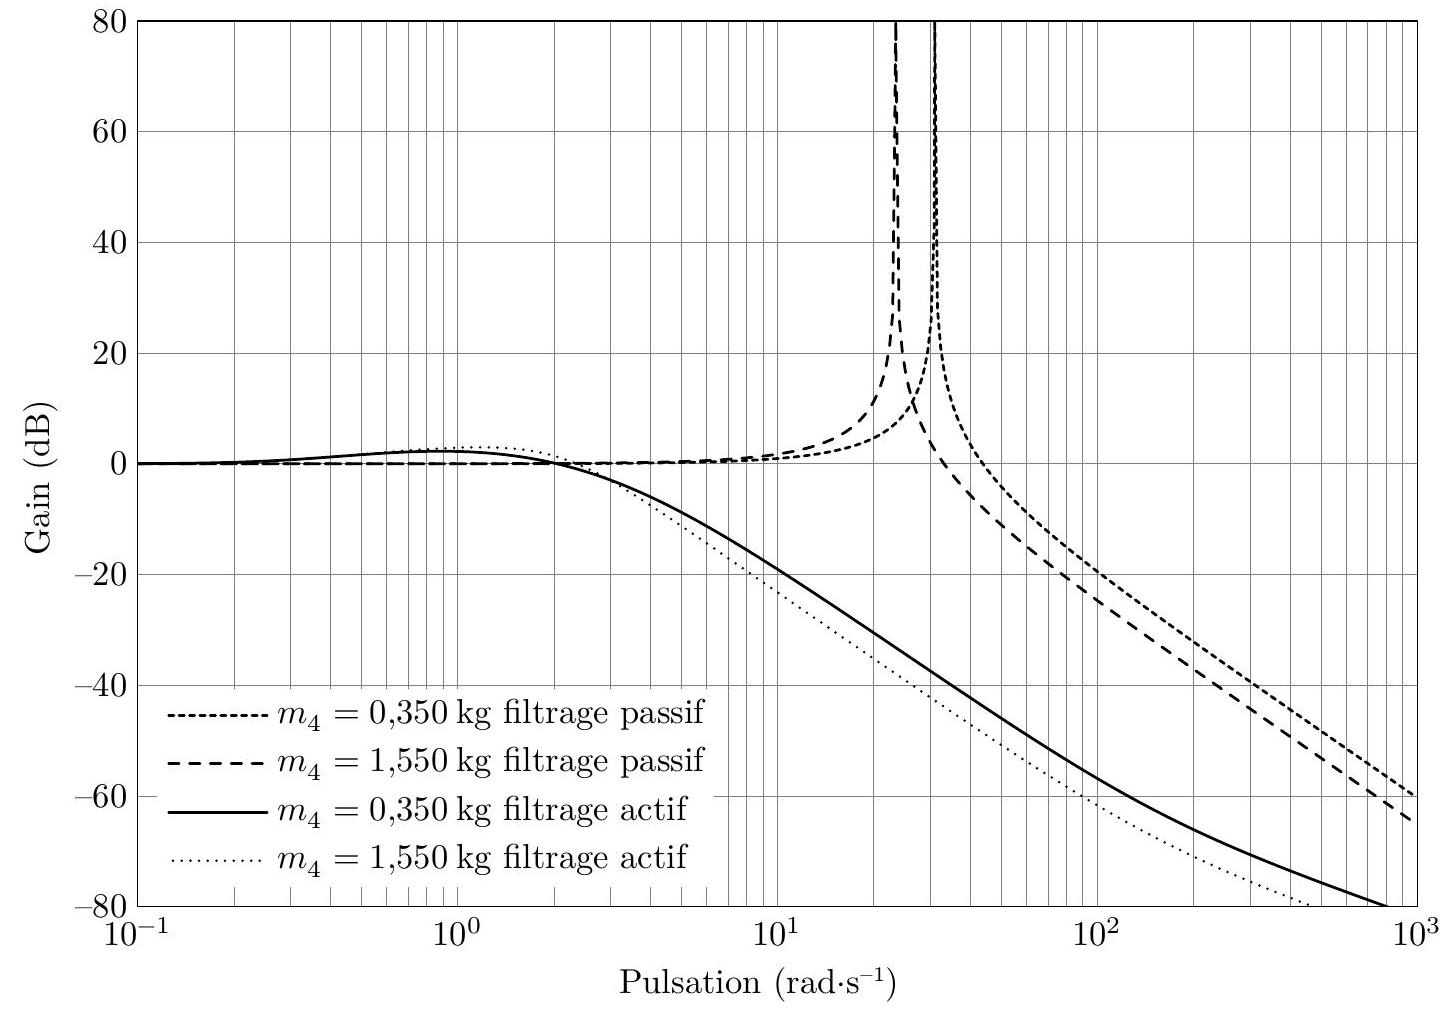
\includegraphics[width=.8\textwidth]{fig_15.jpg}
\caption{\label{fig:15}  Diagrammes de Bode de la fonction $Z_{G}(p) / Z_{\text {pert }}(p)$}
\end{figure}
\fi


%Q 27. 
\question{\label{q:27} En étudiant les réponses harmoniques (figure~\ref{fig:15}), analyser la pertinence de chacune des deux solutions technologiques étudiées à satisfaire l'exigence 1.2.1.}
\ifprof
\begin{corrige}
Entre \SI{1,5}{Hz} et \SI{2,8}{Hz}, c'est à dire entre \SI{10}{rad.s^{-1}} et \SI{20}{rad.s^{-1}} l'atténuation doit être supérieure à \SI{16}{dB}. Seul le dispositif actif permet de respecter cette exigence. 


Le dispositif passif atténue la perturbation à partir de \SI{40}{rad.s^{-1}} soient 6 pas par seconde, ce qui constitue un rythme de marche élevée.

En conclusion, il semble que le dispositif passif aura des difficultés à stabiliser l'appareil si le preneur de vu marche. En revanche, si les perturbations ont une fréquence plus haute (par exemple si le preneur de vu est sur ou dans un véhicule) le dispositif passif permettra de rejeter les perturbations. 

\end{corrige}
\else
\fi

 %Q 28. 
\question{\label{q:28}En considérant des critères de respect des performances attendues, d'encombrement, de masse, de coût et de consommation d'énergie, établir un tableau comparatif et argumenter un choix entre les deux solutions.}
\ifprof
\begin{corrige}
\begin{center}
\begin{tabular}{p{3.5cm}ccp{7cm}}
\cline{2-4}
 & Filtrage actif & Filtrage passif & Remarques \\ \hline \hline
 Performances CDC & \smiley &\frownie{}& \\ \hline
 Encombrement  &\frownie{}& \smiley&  La motorisation ajoute des composants qui peuvent nuire à l’encombrement. \\ \hline
 Masse  &\frownie{}&\smiley &La motorisation ajoute des composants qui vont augmenter la masse. \\ \hline
 Coût  &\frownie{} & \smiley& La motorisation ajoute des composants qui vont augmenter le coût. \\ \hline
 Consommation d'énergie  &\frownie{} & \smiley& La motorisation consommera davantage d'énergie qu'un système entièrement passif sans actionneur supplémentaire. \\ \hline
\end{tabular}
\end{center}

Si l'utilisateur est très exigeant sur les performances attendues du produit, il devra opter pour un filtrage actif. 


\end{corrige}
\else
\fi


\ifprof
\else
\begin{figure}[H]
\centering
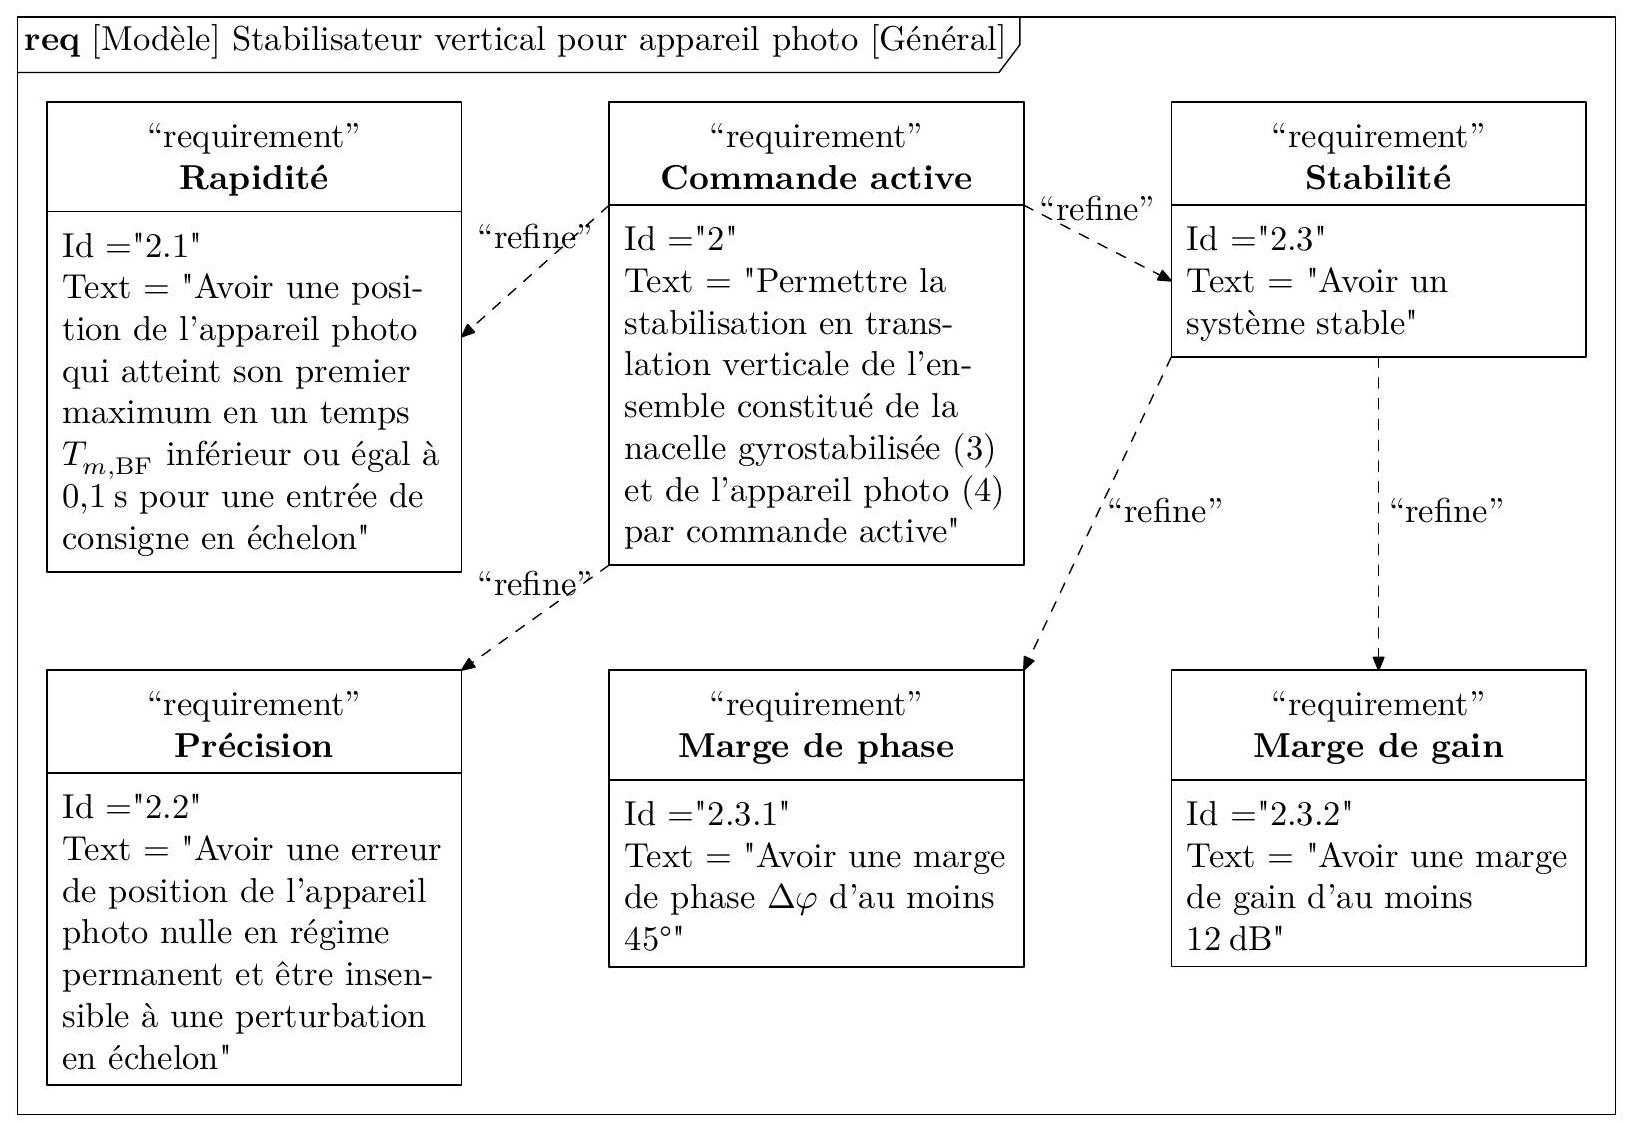
\includegraphics[width=\textwidth]{fig_16.jpg}
\caption{\label{fig:A}  Extrait du cahier des charges fonctionnel}
\end{figure}

\begin{figure}[H]
\centering
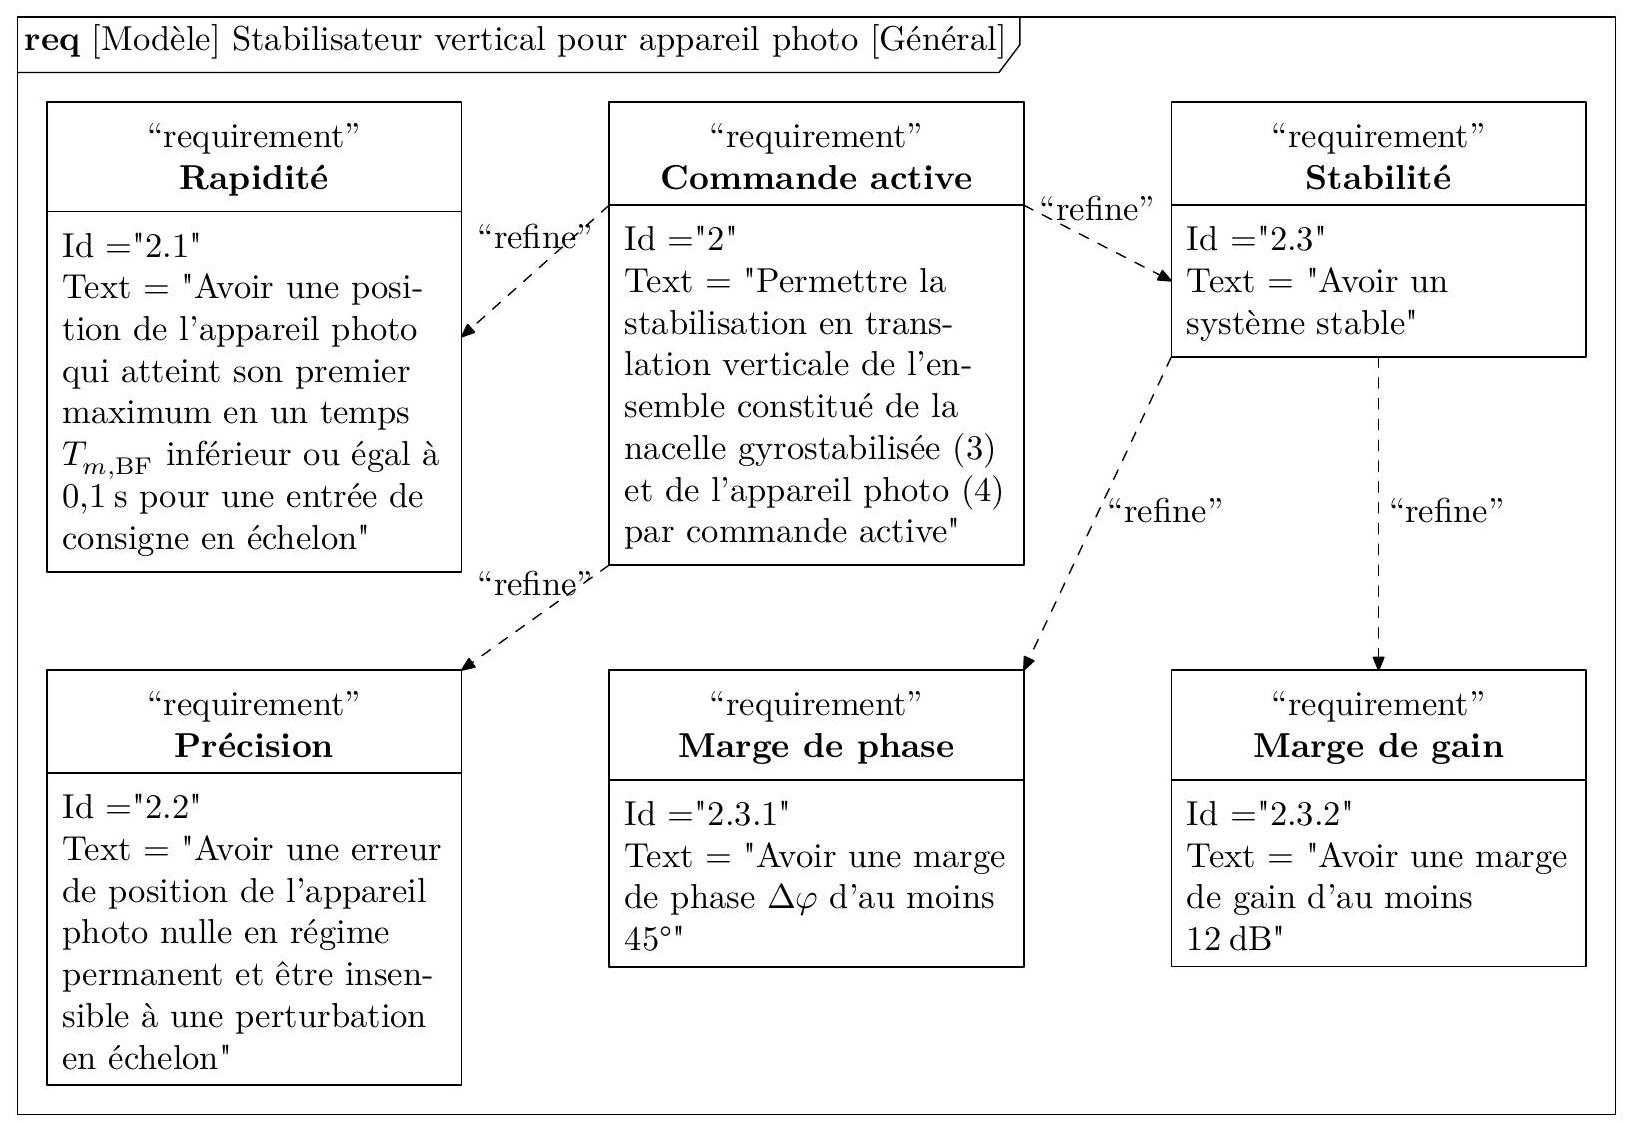
\includegraphics[width=\textwidth]{fig_17.jpg}
\caption{\label{fig:B} Diagramme des exigences partiel du stabilisateur vertical avec la commande active}
\end{figure}


\begin{figure}[H]
\centering
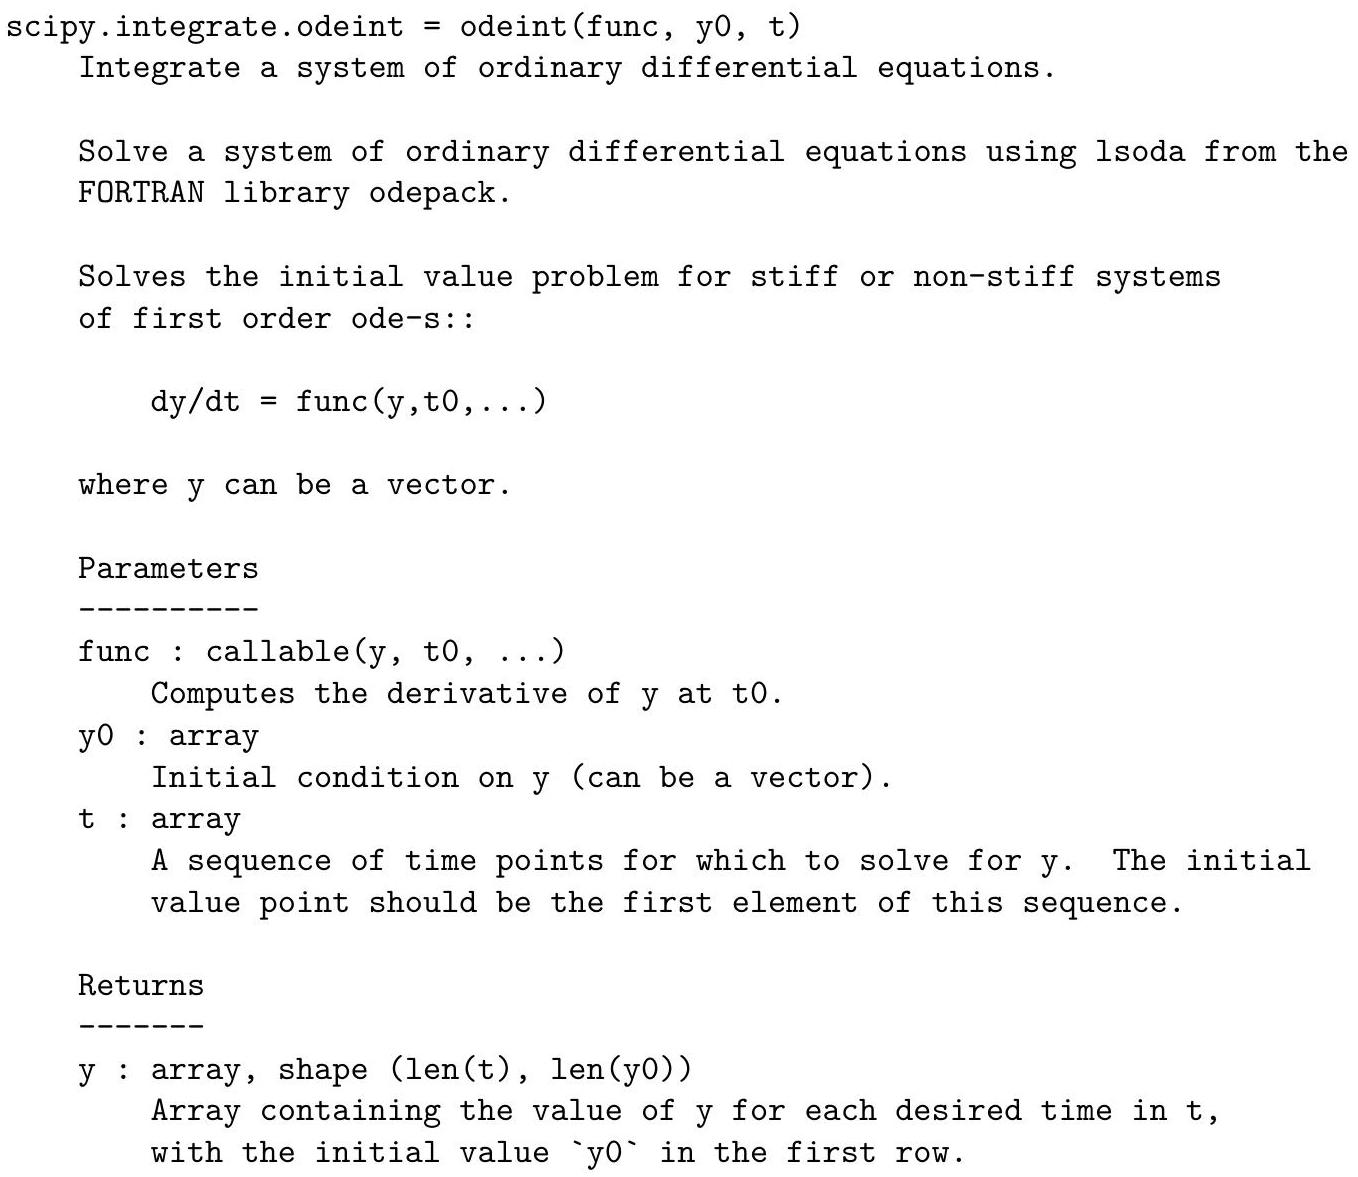
\includegraphics[width=.8\textwidth]{fig_19.jpg}
\caption{\label{fig:D} Extrait de l’aide sur la fonction Python scipy.integrate.odeint}
\end{figure}
\fi